\let\negmedspace\undefined
\let\negthickspace\undefined
\documentclass[journal]{IEEEtran}
\usepackage[a5paper, margin=10mm, onecolumn]{geometry}
\usepackage{lmodern} % Ensure lmodern is loaded for pdflatex
\usepackage{tfrupee} % Include tfrupee package

\setlength{\headheight}{1cm} % Set the height of the header box
\setlength{\headsep}{0mm}     % Set the distance between the header box and the top of the text

\usepackage{gvv-book}
\usepackage{gvv}
\usepackage{cite}
\usepackage{amsmath,amssymb,amsfonts,amsthm}
\usepackage{algorithmic}
\usepackage{graphicx}
\usepackage{textcomp}
\usepackage{xcolor}
\usepackage{txfonts}
\usepackage{listings}
\usepackage{enumitem}
\usepackage{mathtools}
\usepackage{gensymb}
\usepackage{comment}
\usepackage[breaklinks=true]{hyperref}
\usepackage{tkz-euclide} 
\usepackage{listings}
\usepackage{gvv}                                        
\def\inputGnumericTable{}                                 
\usepackage[latin1]{inputenc}                                
\usepackage{color}                                            
\usepackage{array}                                            
\usepackage{longtable}                                       
\usepackage{calc}                                             
\usepackage{multirow}                                         
\usepackage{hhline}                                           
\usepackage{ifthen}                                           
\usepackage{lscape}
\begin{document}

\bibliographystyle{IEEEtran}
\vspace{3cm}

\title{9.5.17.1}
\author{EE24BTECH11003 - Akshara Sarma Chennubhatla}
% \maketitle
% \newpage
% \bigskip
{\let\newpage\relax\maketitle}
\textbf{Question:}
Solve the differential equation $\brak{4x + 6y + 5}dy - \brak{3y + 2x + 4}dx = 0$, with initial conditions $x_0 = 0, y_0 = 0$\\

\solution\\
\textbf{Theoretical Solution:}\\

\begin{align}
	\brak{3y + 2x + 4}dx &= \brak{4x + 6y + 5}dy\\
	\frac{dy}{dx} &= \frac{\brak{3y + 2x + 4}}{\brak{4x + 6y + 5}}\\
\end{align}
Taking $2x + 3y$ as $t$
\begin{align}
	2 + 3 \frac{dy}{dx} &= \frac{dt}{dx}\\
	\frac{t + 4}{2t + 5} &= \frac{1}{3}\brak{\frac{dt}{dx} - 2}\\
	\frac{7t + 22}{2t + 5} &= \frac{dt}{dx}\\
\end{align}
Integrating on both sides,
\begin{align}
	\int dx &= \int \frac{2t + 5}{7t + 22}dt\\
	x &= \frac{2}{7}\brak{t - \frac{9}{14}\log\brak{14t + 44}} + C\\
	x &= \frac{2}{7}\brak{2x + 3y - \frac{9}{14}\log\brak{28x + 42y + 44}} + C\\
	x_0 &= 0, y_0 = 0,\\
	3x &= 6y - \frac{9}{7}\log\brak{\frac{28x + 42y + 44}{44}}\\
\end{align}

\textbf{Simulated Solution:}\\

By first principle of derivatives,
\begin{align}
	y^{\prime}\brak{x} = \lim_{h\to 0}\frac{y\brak{x+h} - y\brak{x}}{h}\\
	y\brak{x+h} = y\brak{x} + hy^{\prime}\brak{x}
\end{align}

Given differential equation can be written as,
\begin{align}
	y\prime = \frac{3y + 2x + 4}{4x + 6y + 5}   
\end{align}

So, by using the method of finite diffferences,
\begin{align}
	y_1 = y_0 + h \brak{\frac{3y_0 + 2x_0 + 4}{4x_0 + 6y_0 + 5}}
\end{align}
Similarly, by iterating for $y_2, y_3$...,
The general difference equation is:
\begin{align}
	y_{n+1} = y_n + h \brak{\frac{3y_n + 2x_n + 4}{4x_n + 6y_n + 5}}
\end{align}

Below is the simulated plot and the theoretical plot for given curve  based on initial conditions, obtained by iterating through the values of $x$ with step size of $h$
\begin{figure}[h!]
	\centering
	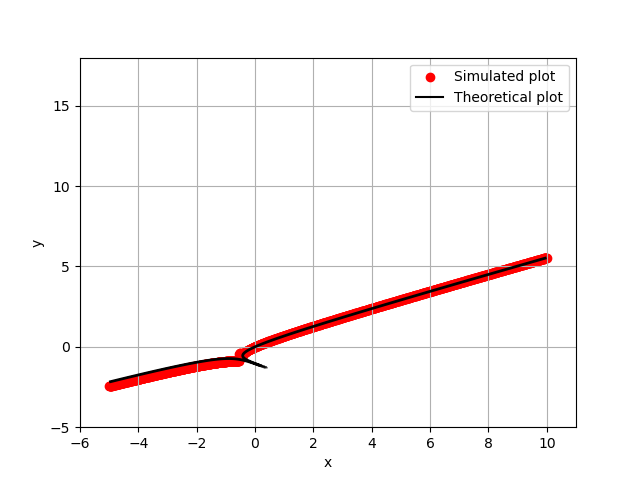
\includegraphics[width=1\columnwidth]{figs/simulated.png}
	\caption{Plot of the solution of $\brak{4x + 6y + 5}dy - \brak{3y + 2x + 4}dx = 0$}
	\label{stemplot}
\end{figure}

\end{document}
